\documentclass[unicode,aspectratio=169,11pt]{beamer}
\usepackage{amsmath, amssymb, amsthm, color, latexsym, mathrsfs, bm}
\usefonttheme{professionalfonts}
\usepackage{luatexja}
\usepackage[ipaex]{luatexja-preset}
\renewcommand{\kanjifamilydefault}{\gtdefault}

\usetheme[
  sectionpage=none,
  numbering=fraction,
  block=fill
  ]{metropolis}

\title{
    The AI economist:
    Improving Equality and Productivity with AI-Driven Tax Policies
}
\subtitle{Stephan Zheng, Alexander Trott, Sunil Srinivasa, Nikhil Naik, Melvin Gruesbeck, David C. Parkes, and Richard Socher, 2020, mimeo.}
\author{Presenter: Yoji Tomita}
\date{RL-GTゼミ June 17, 2021}

\begin{document}

\maketitle

\begin{frame}{Table of Contents}
    \tableofcontents
\end{frame}

\section{1. Introduction}
\begin{frame}{1. Introduction}
    \begin{itemize}
        \item イントロダクション
    \end{itemize}
\end{frame}

\section{2. Economic Simulations: Learning in Gather-and-Build Games}

\begin{frame}{2. Economic Simulations: Learning in Gather-and-Build Games}{}
    \begin{itemize}
        \item Economic environmentについて.
        \item まずは税の無い設定("free-market")で説明する.
    \end{itemize}
\end{frame}

\subsection{2.1 Notation and Preliminaries}
\begin{frame}{2.1 Notation and Preliminaries}
    \begin{itemize}
        \item Partial-observable multi-agent Markov Games(MGs): $(S, A, r, \mathscr{T}, \gamma, o, \mathscr{I})$
        \begin{itemize}
            \item $S$ : 状態空間(state space)
            \item $A$ : 行動空間(action space)
            \item $r_{i,t}$ : 報酬関数(reward function)
            \item $\mathscr{T}$ : 遷移関数(transition function)  $s_{t+1} \sim \mathscr{T}(\cdot \mid s_t, \bm{a}_t)$
            \item $\gamma$ : 割引因子(discount factor)
            \item $o_{i,t}$ : 観測(observation)
            \item time step $t = 0, 1, \dots, H$.
        \end{itemize}
    \end{itemize}
\end{frame}

\begin{frame}{}{}
\begin{itemize}
    \item Agents' policy : $\pi_i(\cdot \mid o_{i,t}, h_{i,t}; \theta_i)$
    \begin{itemize}
        \item $h_{i,t}$ : hidden state(自分の私的情報と, 過去のhistory)
        \item $\theta_i$ : policyのparameter
        \item エージェント $i$ は次の最大化問題を得くpolicyを求める:
        \[
            \max_{\theta_i} \mathbb{E}_{a_i \sim \pi_i, \bm{a}_{-i} \sim \bm{\pi}_{-i}, s'\sim \mathscr{T}}\left[\sum_{t}\gamma^t r_{i,t}\right].
            \tag{1}
        \]
    \end{itemize}
     
    \item データ効率性のため, すべてのエージェントはtrainingの間パラメータ$\theta$を共有する.
    \item 彼らの行動 $\pi_i(a_i\mid o_i, h_i; \theta)$ は, agent-specific observations $o_i$ と hidden-state $h_i$によって異なる.
\end{itemize}
\end{frame}

\begin{frame}
    \begin{center}
        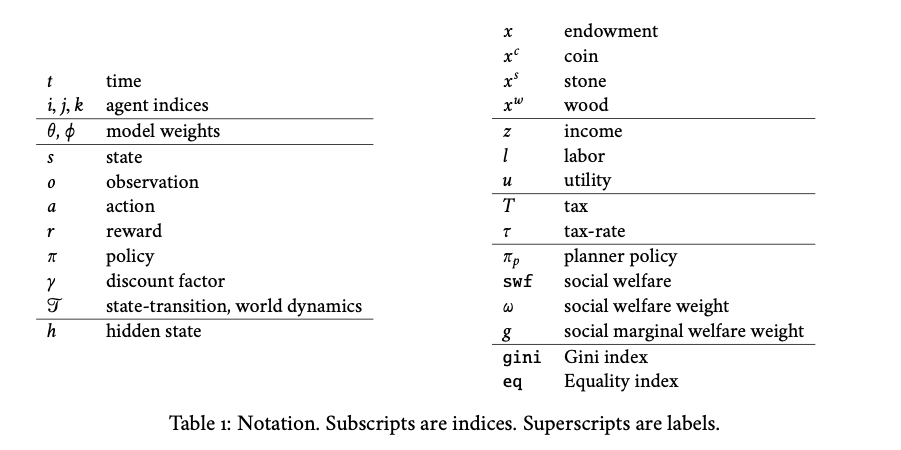
\includegraphics[width=15cm]{table1.png}
    \end{center}
\end{frame}

\subsection{2.2 Environment Rules and Dynamics}
\begin{frame}{2.2 Environment Rules and Dynamics}{}
{\bf Gather-and-Build game}
\begin{itemize}
    \item 2次元のgrid ($25 \times 25$) からなる世界が舞台.
    \item エージェントはフィールドを歩き回り, 資源(石と木)を集め, それらを1つずつ使って家を建て, また資源をcoinを介してトレードする.
    \item 資源は空タイルに確率的に産み出される.
    \item エージェントは家を建てるとcoinが得られるが, 得られるcoinはagentのskillごとに異なる.
\end{itemize}
\end{frame}

\begin{frame}{}{}
{\bf Labor and Skill.}
\begin{itemize}
    \item Agentのaction(moving, gathering, trading, building)にはそれぞれlabor costが設定されている.
    \item 各timeにagentがどれか1つ行動をとると, そのlabor costがかかる.\\
     
    \item building skill (1以上3以下)が各agentに設定されていて, 家を建てるとagentは $10 \times$ skill 分のcoinを得る.
    \item collection skill (1以上2以下)もあり, 資源を拾うとこのskill分の資源を得る\\
          (skill 1.2 の場合, 確定で1つ資源を得て, さらに確率0.2でもう1つ資源を得る)
\end{itemize}
\end{frame}

\begin{frame}{}{}
{\bf Environment Scenario.}
\begin{columns}[t]
    \begin{column}{0.6\textwidth}
        \begin{itemize}
            \item fieldは水により4つの区域に別れている(水部分は通れない)
            \item 資源は空間的に集まって発生する.
            \item 4 agents
            \item buildng skills は 1.13, 1.33, 1.65, 22.2(Pareto分布 w/ exponent $a=4$, scale $m=1$のquartilesを元に設定)
            \item 1 episodeは$H = 1000$ time stepsからなる.
        \end{itemize}
    \end{column}
    \begin{column}{0.4\textwidth}
        \begin{center}
            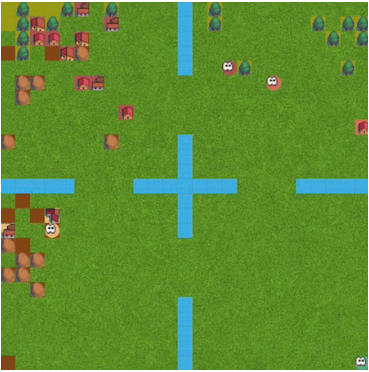
\includegraphics[width=5cm]{figure1.png}
        \end{center}
    \end{column}
\end{columns}
\end{frame}

\subsection{2.3 Using Machine Learning to Optimize Agent Behavior}
\begin{frame}{2.3 Using Machine Learning to Optimize Agent Behavior}{}
    \begin{itemize}
        \item Agentのutility function:
        \[
            u_i(x_{i,t}, l_{i,t}) = \mathrm{crra}\left(x_{i,t}^c \right) - l_{i,t},
            \ \ \ \mathrm{where}\ \ \mathrm{crra}(z) = \frac{z^{1-\eta} - 1}{1-\eta},\ \ \eta>0.
            \tag{2}
        \]
        \begin{itemize}
            \item $x_{i,t} = (x_{i,t}^w, x_{i,t}^s, x_{i,t}^c)$: $i$の保有する木・石・コイン.
            \item $l_{i,t}$: 蓄積労働量.
            \item $\eta$: エージェントのutility functionのnon-linearityをコントロールするパラメータ.
        \end{itemize}
        \item Rational economic agentは以下の最大化を行う.
        \[
            \forall i : \max_{\pi_i} \mathbb{E}_{a_i \sim \pi_i,\ \bm{a}_{-i}\sim \bm{\pi}_{-i}, s'\sim \mathscr{T}}
            \left[u_i(x_{i,0}, l_{i,0}) + \sum_{t=1}^H\gamma^t \underbrace{\left(u_i(x_{i,t}, l_{i,t})-u_i(x_{i,t-1}, l_{i,t-1})\right)}_{=r_{i,t}}\right].
            \tag{3}
        \]
    \end{itemize}
\end{frame}

\begin{frame}{}{}
{\bf Deep RL agents}
\begin{itemize}
    \item deep neural networkを用いるagent policyをmodellingする:
    \[ a_{i,t} \sim \pi(o^{\mathrm{world}}_{i,t}, o^{\mathrm{agent}}_{i,t}, o^{\mathrm{market}}_{i,t}, o^{\mathrm{tax}}_{i,t}, h_{i,t-1};\theta) \]
    \begin{itemize}
        \item $o^{\mathrm{world}}_{i,t}$: 近くの状況に関する観測.
        \item $o^{\mathrm{agent}}_{i,t}$: publicなagentの状況(資源・コイン保有)と, private agent states(skill値とlabor performed)
        \item $o^{\mathrm{market}}_{i,t}$: transfer marketの状況(bid, ask offer)
        \item $o^{\mathrm{tax}}_{i,t}$: tax rates
    \end{itemize}
\end{itemize}
\end{frame}

\begin{frame}{}{}
    \begin{center}
        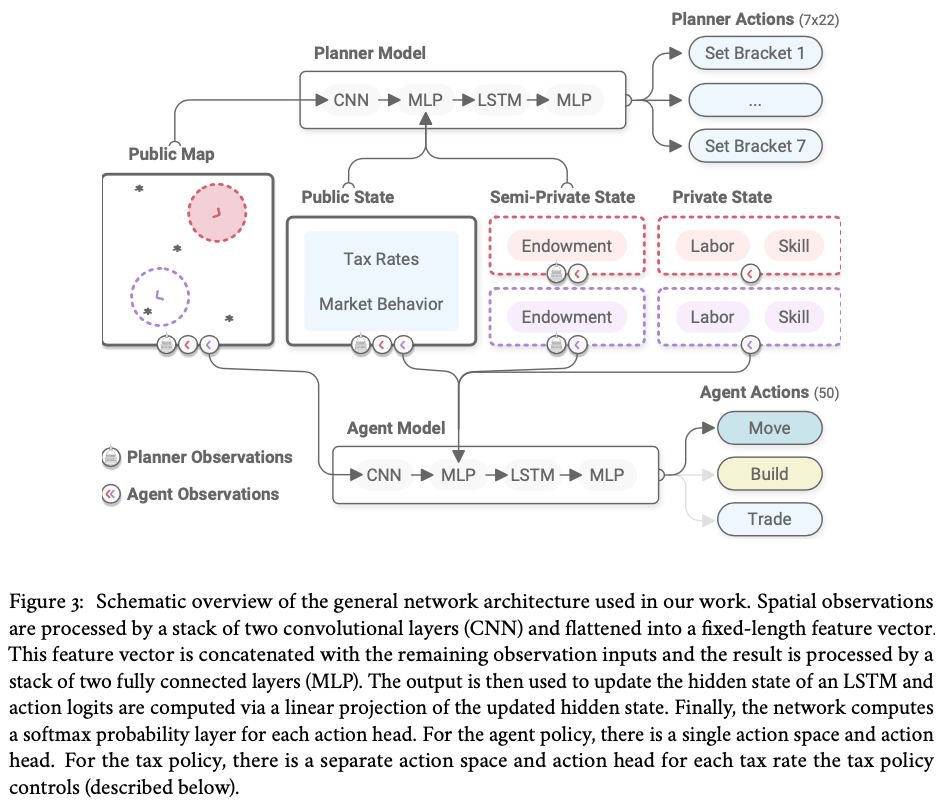
\includegraphics[width=10.3cm]{figure3.png}
    \end{center}
\end{frame}

\begin{frame}{}{}
    {\bf Emergent Behavior of AI Agents}
\begin{columns}[t]
    \begin{column}[]{0.6\textwidth}
        \begin{center}
            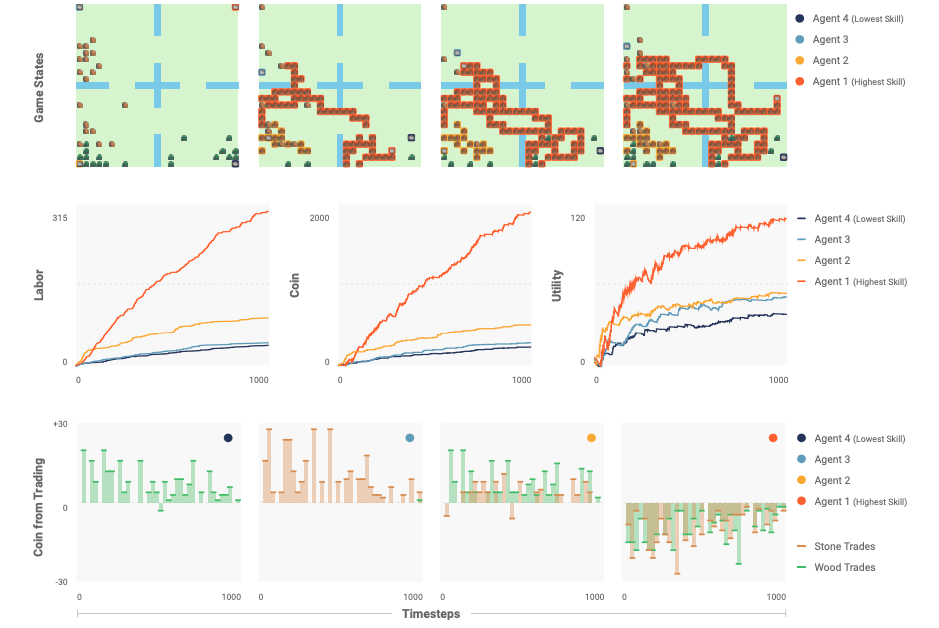
\includegraphics[width=9cm]{figure4.png}
        \end{center}
    \end{column}
    \begin{column}[]{0.4\textwidth}
        \begin{itemize}
            \item 左図はno-tax下でtrain後のAI agentsの1 episodeの行動の例.
            \item low-skill agents(紺,水)は資源を集めてmarketで売ることに徹している.
            \item high-skill agent(オレンジ)はmarketで資源を買って家を建てている.
            \item 黄色は最初は家を建ててるが, のちに資源を得る方にスイッチしている.
        \end{itemize}
    \end{column}
    
\end{columns}
\end{frame}

\section{3. Machine Learning for Optimal Tax Policies}
\begin{frame}{3. Machine Learning for Optimal Tax Policies}
    \begin{itemize}
        \item 課税と再分配を行う social planner を導入する.
        \item Social plannerは, 生産性と平等性のtrade-offに直面している.
        \begin{itemize}
            \item 無課税(free-market)では生産性は最大化されるが, 不平等.
            \item 課税・再分配を行うと平等性が増すが, 生産性が落ちる.
        \end{itemize}
         \\
        \item ここでは, free-market, US-federal, Saez framework, AI economistによるsocial plannerを試す.
    \end{itemize}
\end{frame}

\subsection{3.1 Periodic Taxes with Bracketed Schedules}
\begin{frame}{3.1 Periodic Taxes with Bracketed Schedules}{}
{\bf Income Taxes.}
    \begin{itemize}
        \item Tax periodは $M$ steps続く(実験では$M = H/10$とし, 1 episodeに10 tax periodsがあるものとする)
        \item ピリオド $p$ の税は, time step $t$ から $t + M$ までの収入 $z_i^p$ に課される.\\
                 
        \item Tax periodの初めに, social plannerはtax schedule $T(z)$ を決めて公表する.
        \begin{itemize}
            \item 各agent $i$ は, 収入 $z_i^p$ に応じて $T(z)$ を支払う.
            \item 集められた税は, 全agentに平等に分配される.
            \item よって, 分配後のagent $i$ の収入は,
            \[ \tilde{z}_i^p = z_i^p - T(z_i^p) + \frac{1}{N}\sum_{j=1}^N T\left(z_j^p\right). \tag{5}\]
        \end{itemize}
    \end{itemize}
\end{frame}

\begin{frame}{}{}
{\bf Bracketed Tax Schedules.}
\begin{itemize}
    \item Scheme間の比較を可能にするため, tax scheduleは次のように "bracketed" されたもののみを考える.
    \item Cut-off income levels $\{m_b\}_{b = 0}^B$ s.t. $0 = m_0 \le m_1 \le \dots \le m_{B-1}\le m_B = +\infty$ が先に与えられている.
    \item Social plannerは, 各bracket $b$ に含まれる収入に対して適用されるmarginal tax rate $\tau_b \in [0,1]$を選ぶことで, tax schedule $T(\cdot)$ を決定する.
    \[ T(z) = \sum_{b = 0}^{B-1} \tau_b \cdot \left((m_{b+1}-m_{b}) \cdot 1[z > m_{b+1}] + (z - m_b)\cdot 1[m_b < z \le m_{b+1}]\right).\]
\end{itemize}
\end{frame}

\begin{frame}{3.2 Optimal Taxation}{}
{\bf Social Welfare Functions}
\begin{itemize}
    \item Social plannerの目的関数であるsocial welfare functionは, 生産性と平等性のtrade-offを組み込めるように次のように決める.
    \item エージェントのコイン保有 $\bm{x}^c = (x_1^c, \dots, x_N^c)$ に対し, equalityを次で定義:
    \[ {\bf{eq}}(\bm{x}^c) = 1 - {\bf{gini}}(\bm{x}^c)\cdot \frac{N}{N-1},\ \ \ 0 \le {\bf eq}(\bm{x}^c)\le 1.\tag{7} \]
    where
    \[ {\bf{gini}}(\bm{x}^c) = \frac{\sum_{i=1}^N\sum_{j=1}^N |x_{i}^c - x_{j}^c|}{2N \sum_{i=1}^N x_{i}^c},
    \ \ \ 0 \le {\bf gini}(\bm{x}^c) \le \frac{N-1}{N}\tag{8} \]
    \begin{itemize}
        \item ${\bf eq}$は, $1$で完全に平等(全員同じ収入), $0$で完全に不平等(1人が全コインを独占).
    \end{itemize}
\end{itemize}
\end{frame}

\begin{frame}{}{}
    \begin{itemize}
        \item 生産性は, 
        \[ {\bf prod}(\bm{x}^c) = \sum_{i=1}^N x_{i}^c. \tag{9} \]
        \item この ${\bf eq}$ と ${\bf prod}$ をsocial welfare functionとする.\footnote{Social welfare functionとして, weight $\omega_i \ge 0$ を用いて
        \[ {\bf swf}_t(\bm{x}_t^c, \bm{l}_t) = \sum_{i = 1}^N \omega_i \cdot u_i\left(x_{i,t}^c, l_{i,t}\right). \tag{11}\]
        を用いることも可能.}
        \[ {\bf swf}_t(\bm{x}_t^c) = {\bf eq}_t(\bm{x}_t^c) \cdot {\bf prod}_t (\bm{x}_t^c). \tag{10}\]
    \end{itemize}
\end{frame}

\begin{frame}{}{}
{\bf The Planner's Problem.}
\begin{itemize}
    \item Social Plannerは,
    \begin{itemize}
        \item agentの保有資源・コイン $\bm{x}_{i,t}$, フィールドの状態(agent・資源の位置)とmarketの状況は観測可能,
        \item 各agentのskillは直接には観測できない.
    \end{itemize}
    \item Plannerの最大化問題は,
    \[ \max_{\pi_p} \mathbb{E}_{\tau \sim \pi_p, \bm{a} \sim \bm{\pi}, s'\sim \mathscr{T}}\left[{\bf swf}_0+\sum_{t=1}^H\gamma^t\underbrace{({\bf swf}_t-{\bf swf}_{t-1})}_{=r_{p,t}}\right]. \tag{12} \]
\end{itemize}
\end{frame}

\subsection{3.3 Inner-Outer-Loop Reinforcement Learning}
\begin{frame}{3.3 Inner-Outer-Loop Reinforcement Learning}{}
    \begin{columns}[t]
        \begin{column}[]{0.6\textwidth}
            \begin{center}
                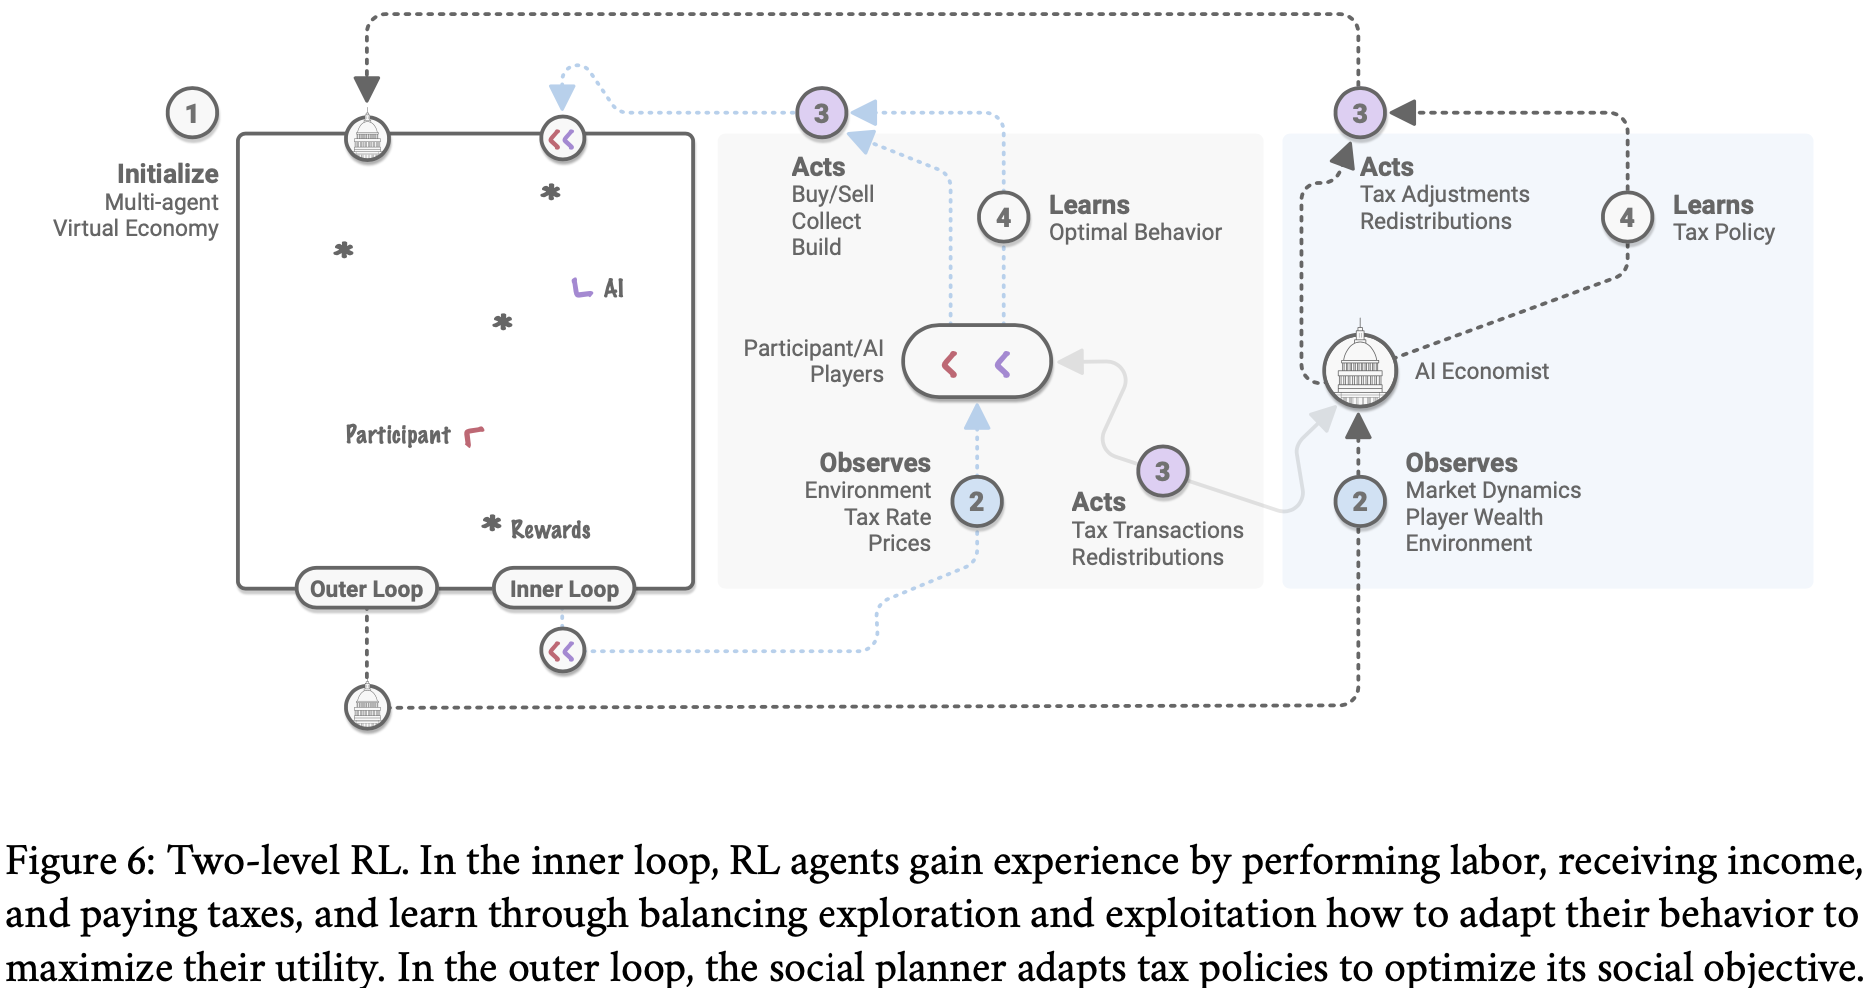
\includegraphics[width=9cm]{figure6.png}
            \end{center}
        \end{column}
        \begin{column}[]{0.4\textwidth}
            \begin{itemize}
                \item この状況では, Inner loopでagentsが行動を選んで学習し, Outer loopでplannerが税制を選んで学習することになる.
                \item Inner loopでのAgentの学習行動と, outer loopでplannerの選ぶ税制が相互に影響し合うため, 報酬がagentとplanner双方にとって不安定になる.
            \end{itemize}
        \end{column}
    \end{columns}
\end{frame}

\begin{frame}
    \begin{center}
        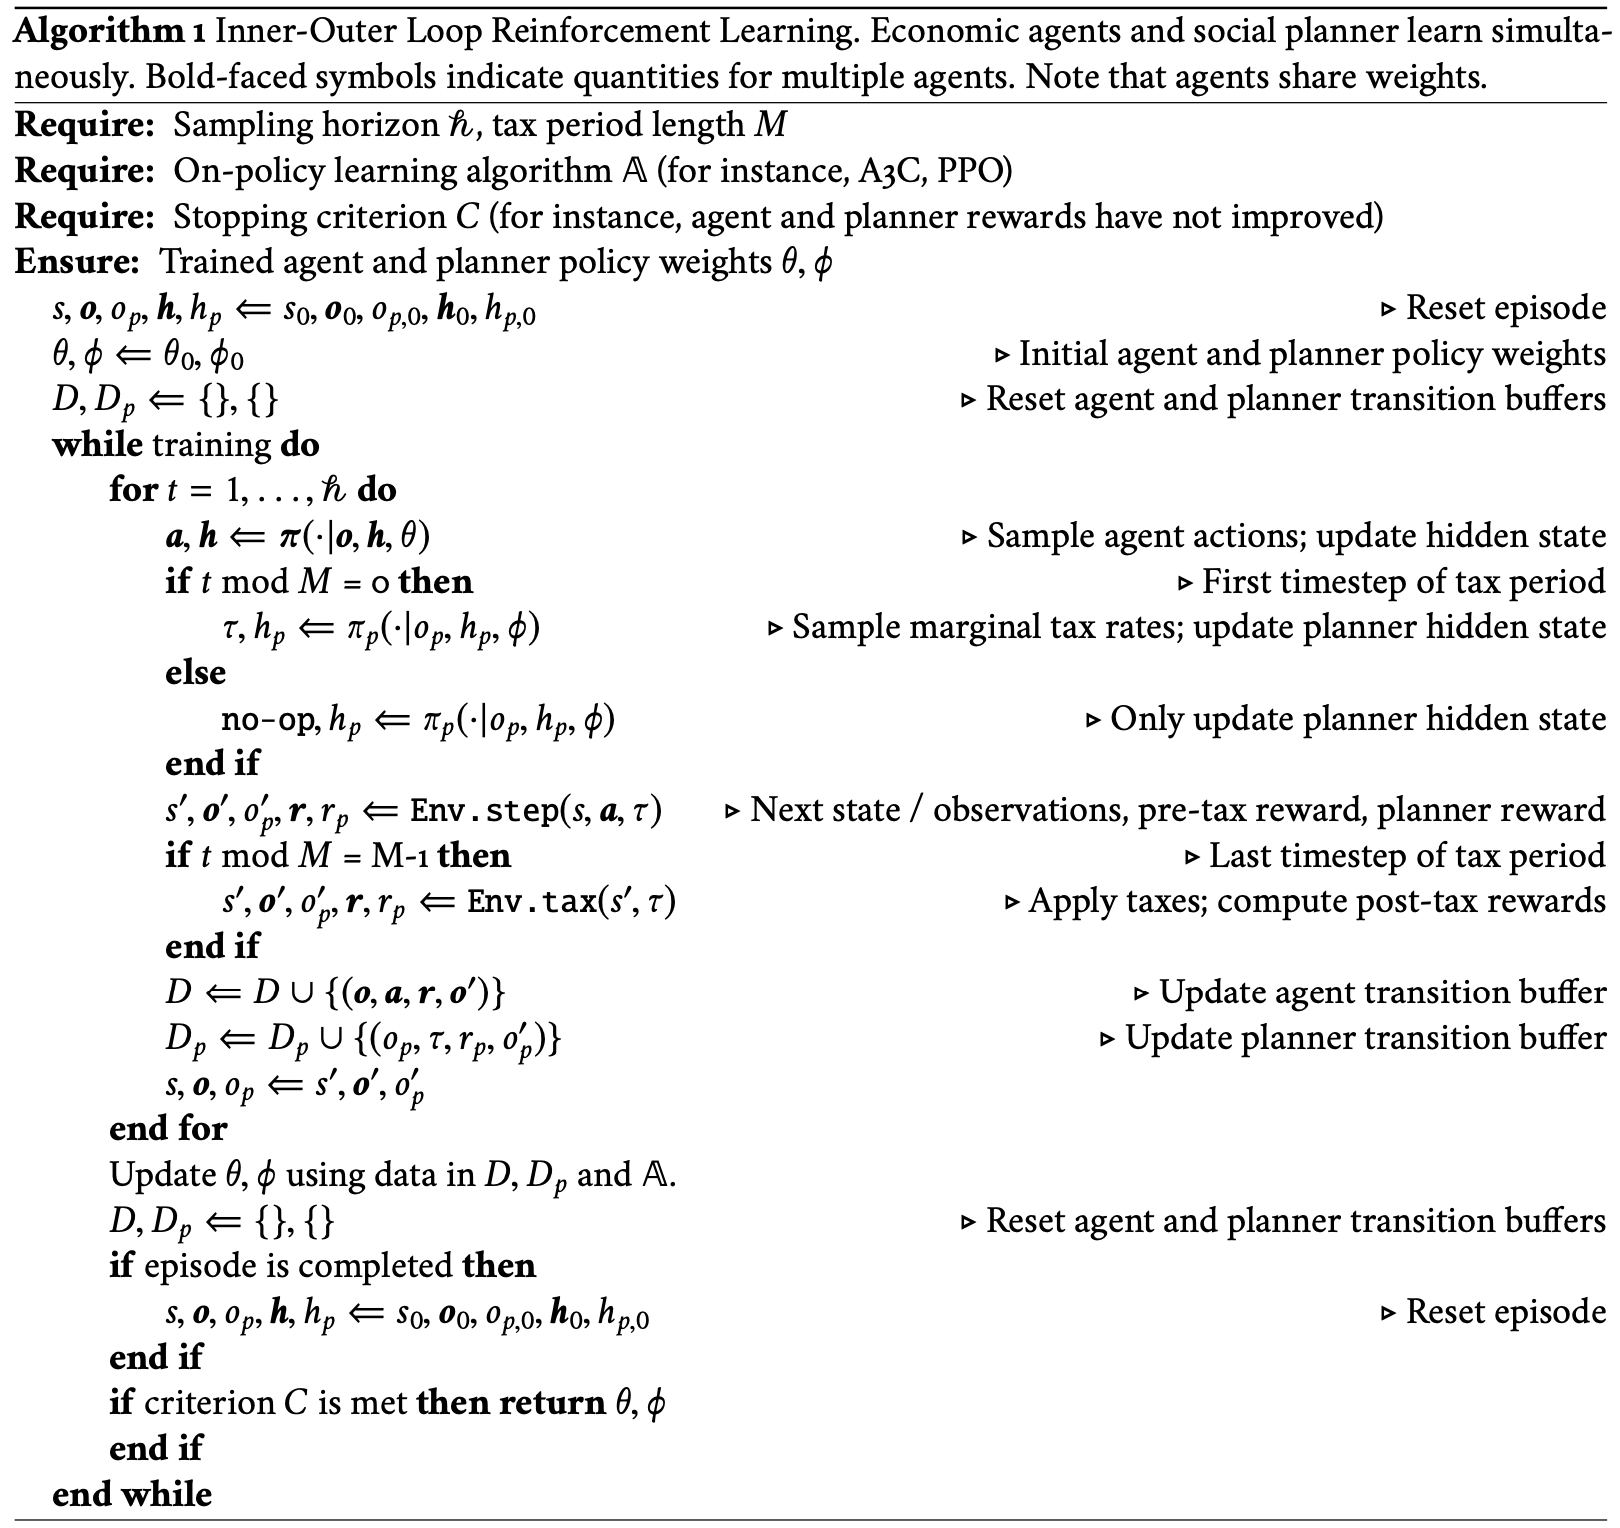
\includegraphics[width=9.3cm]{algorithm1.png}
    \end{center}
\end{frame}

\section{4. Improved Social Outcomes with AI Agents}
\begin{frame}{4. Improved Social Outcomes with AI Agents}{}
{\large\bf 4.1 Baseline Methods}
\begin{itemize}
    \item 次の4つのtax modelを比較する.
    \begin{itemize}
        \item free-market (no taxes)
        \item US federal single-filer 2018 tax schedule
        \item Saez tax formula (adapted for a multi-period setting)
        \item AI Economist planner
    \end{itemize}
    \item Tax bracketは, 全てのtax modelに共通で, 2018 US federal incom taxをもとに1/1000にスケーリングした以下を用いる.
    \[ \bm{m} = [0, 9.7, 39.475, 84.2, 160.725, 204.100, 510.3, \infty]. \tag{15} \]
\end{itemize}
\end{frame}

\begin{frame}{}{}
{\bf US Federal Income Tax Rates (Single-filer, 2018).}
\begin{itemize}
    \item 2018 US federal income taxをもとに, bracket tax ratesは, 
    \[ \bm{\tau} = [0.1, 0.12, 0.22, 0.24, 0.32, 0.35, 0.37] \tag{16} \]
    とする.
\end{itemize}    
\end{frame}

\begin{frame}{}{}
{\bf Saez Tax Formula (single-period)}
\begin{itemize}
    \item Saez [2001]をもとに, まずsingle-period economyでのoptimal tax ratesを求める.
    \item $f, F$は(pre-tax)収入の分布のprobability densityとcummulative distribution functionとし, plannerはそれらを観測できるとする.
    \item Saez [2001]では, まずlinear-weighted social welfare functions (11)に対し, social marginal welfare weights
    \[ g_i = \frac{\mathrm{d}{\bf swf}}{\mathrm{d} u_i} \frac{\mathrm{d} u_i}{\mathrm{d} x_{i}^c} = \omega_i \frac{\mathrm{d} u_i}{\mathrm{d} x_{i}^c}.  \]
    を求める.
    \item これを我々のモデルに当てはめるために$g_i = \frac{1}{z_i}$とし, さらにこれをnormalizeしてよい $\sum_{i \in \mathscr{T}}g_i = 1$.
\end{itemize}
\end{frame}

\begin{frame}{}{}
    \begin{itemize}
        \item $\alpha(z)$を, the marginal average income at income z, normalized by the fraction of incomes above z, つまり,
        \[ \alpha(z) := \frac{z \cdot f(z)}{1 - F(z)}. \tag{18}\]
        \item $G(z)$は, normalized, reverse cumulative Pareto weight over incomes above a threshold z
        \[ G(z) := \frac{1}{1 - F(z)}\int_{z' = z}^\infty f(z')g(z') \mathrm{d}z'. \tag{19}\]
        \item また, 弾力性(elasticity) $e(z)$を, average sensitivity of an agent’s income to changes in the tax rate, つまり
        \[e(z) = \frac{\mathrm{d}z / z}{\mathrm{d}(1 - \tau(z))/(1-\tau(z))}. \tag{20}\]
        \item Saez [2001]によると, optimal marginal tax-rateは
        \[ \tau(z) = \frac{1 - G(z)}{1 - G(z) + \alpha(z) e(z)} \tag{21}\]
        となり, これはincome distributionとelasticityに依存して決まる.
    \end{itemize}
\end{frame}

\begin{frame}{}{}
{\bf Saez Tax Formula (multi-period)}
\begin{itemize}
    \item Saez formula (21) を使うには, income elasticity $e(z)$ の推定が必要.
    \item Gruber and Saez [2002]に従い, constant tax elasticity $\tilde{e}$ を仮定すると, 
    \[ z_t = z^0 \cdot (1- \tau_t)^{\tilde{e}}. \tag{22} \]
    \item したがって, 
    \[ \log(z_t) = \tilde{e} \cdot \log(1 - \tau_t) + \log(z^0) \tag{23} \]
    を過去のtax periodのデータからOLSで推定して用いる.
\end{itemize}
\end{frame}

\begin{frame}{}{}
    \begin{itemize}
        \item AI Economistは, deep neural networkにより各bucketのmarginal tax rateを決める.
        \[ \tau \sim \pi_p\left( o^{\mathrm{world}}_{p,t}, o^{\mathrm{agent}}_{p,t}, o^{\mathrm{market}}_{p,t}, o^{\mathrm{tax}}_{p,t}, h_{p, t-1} ; \phi \right). \tag{24} \]
        \begin{itemize}
            \item Basic network architectureはagentと同様(Figure 3).
            \item agentとplannerは持つobservationが異なる(plannerはフィールド全体が見れるが, agentのprivate skillは見れない).
        \end{itemize}
    \end{itemize}
\end{frame}

\subsection{4.2 Training Strategy: Two-phase Training and Tax Curricula}
\begin{frame}{4.2 Training Strategy: Two-phase Training and Tax Curricula}
\begin{itemize}
    \item Section 3.3で述べたように, このjoint optimizationは不安定性をもたらす.
    \item 学習を安定化させるため, ここでは次のtwo-pahse training approachを行った.
    \begin{itemize}
        \item First phaze: agent modelsの集合に対し, 無課税(no-tax scenario)で学習させる.
        \item Second phaze: 税モデルを融合にし, エージェント・プランナーの学習を継続する.\\
                また突然の税導入による不安定性を回避するため, 限界税率の上限を$10\%$から$100\%$に徐々に引き上げる.
    \end{itemize}
    \item また, planner policyにentropy regularizationを行うことも効果的だった.
    \begin{itemize}
        \item Entropy regularizationは, policy gradient objectiveに次のadditional, weighted term
        \[ {\bf entropy}(\pi) = - \mathbb{E}_{a \sim \pi(\cdot \mid s)} [\log\pi(a \mid s)]. \]
        を加える(Williams and Peng [1991], Mnih et al. [2016]).
    \end{itemize}
\end{itemize}
\end{frame}

\begin{frame}{}{}
\begin{itemize}
    \item 実験はRLlib flamework [Liang et al., 2018]を用いて実施.
    \item またPolicy gradientsの計算に, proximal policy gradients [Schulman et al., 2017]とAdam optimizer [Kingma and Ba, 2014] を使う.
    \item サンプルは60のenvironment replicasから平行して集め, sampling horizonは200 timestepsとする.
    \item 全ての実験で, 400 million sampleのphase two trainingを実施し, これはagentとplanner modelはstable policyへの収束に十分であった.
\end{itemize}
\end{frame}

\subsection{4.3 Equality, Productivity, and Social Welfare Metrics}
\begin{frame}{4.3 Equality, Productivity, and Social Welfare Metrics}{}
    \begin{center}
        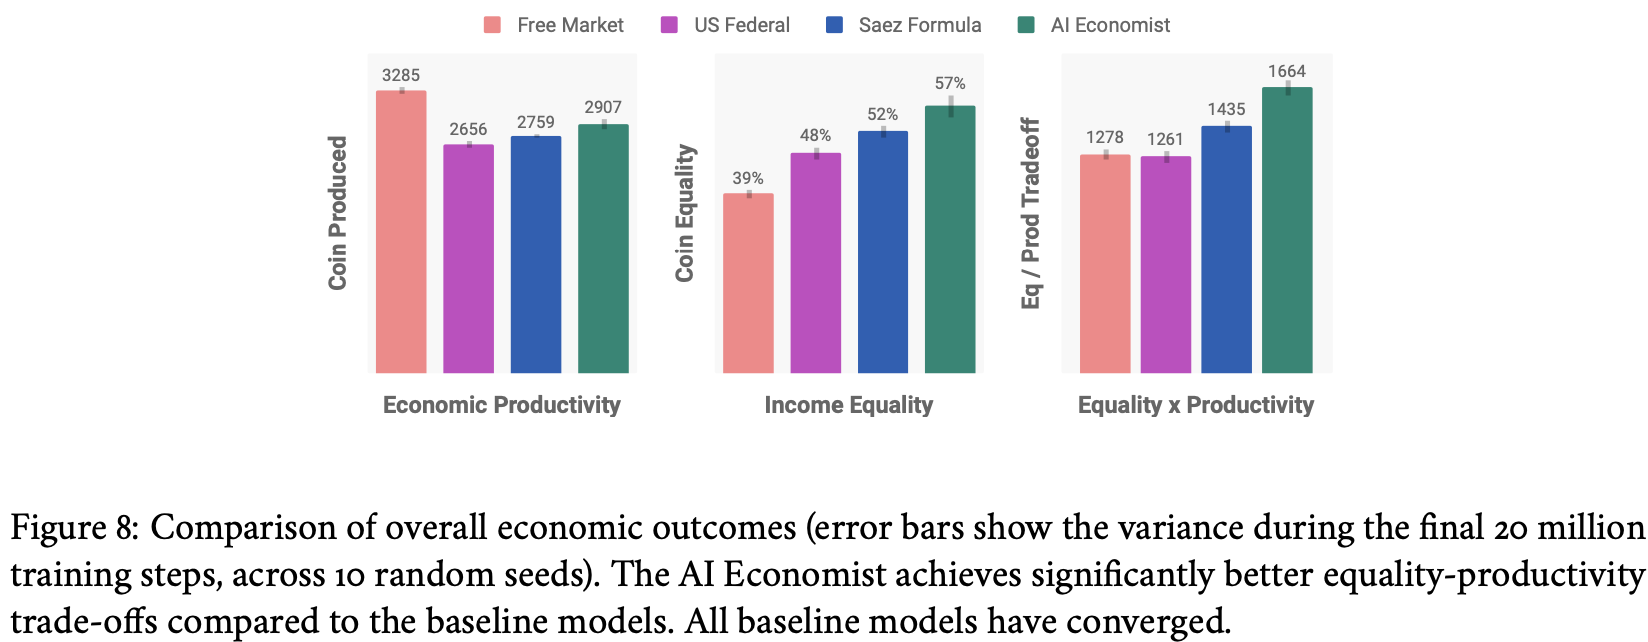
\includegraphics[width=10cm]{figure8.png}
    \end{center}
    \begin{itemize}
        \item Figure 8はepisode終了時の各tax modelでのeconomic outcomesの比較.
        \item Taxは常にproductivityを下げるが, その下り幅はAI Economistが最も少ない.
        \item Income equality($1 - \mathrm{Gini\ index}$)は, AI economistで最も高い.
        \item EqualityとProductivityの積もAI economistが最も高く, 次に高いSaez formulaと比べても$16\%$高い.
    \end{itemize}
\end{frame}

\begin{frame}{}{}
    \begin{center}
        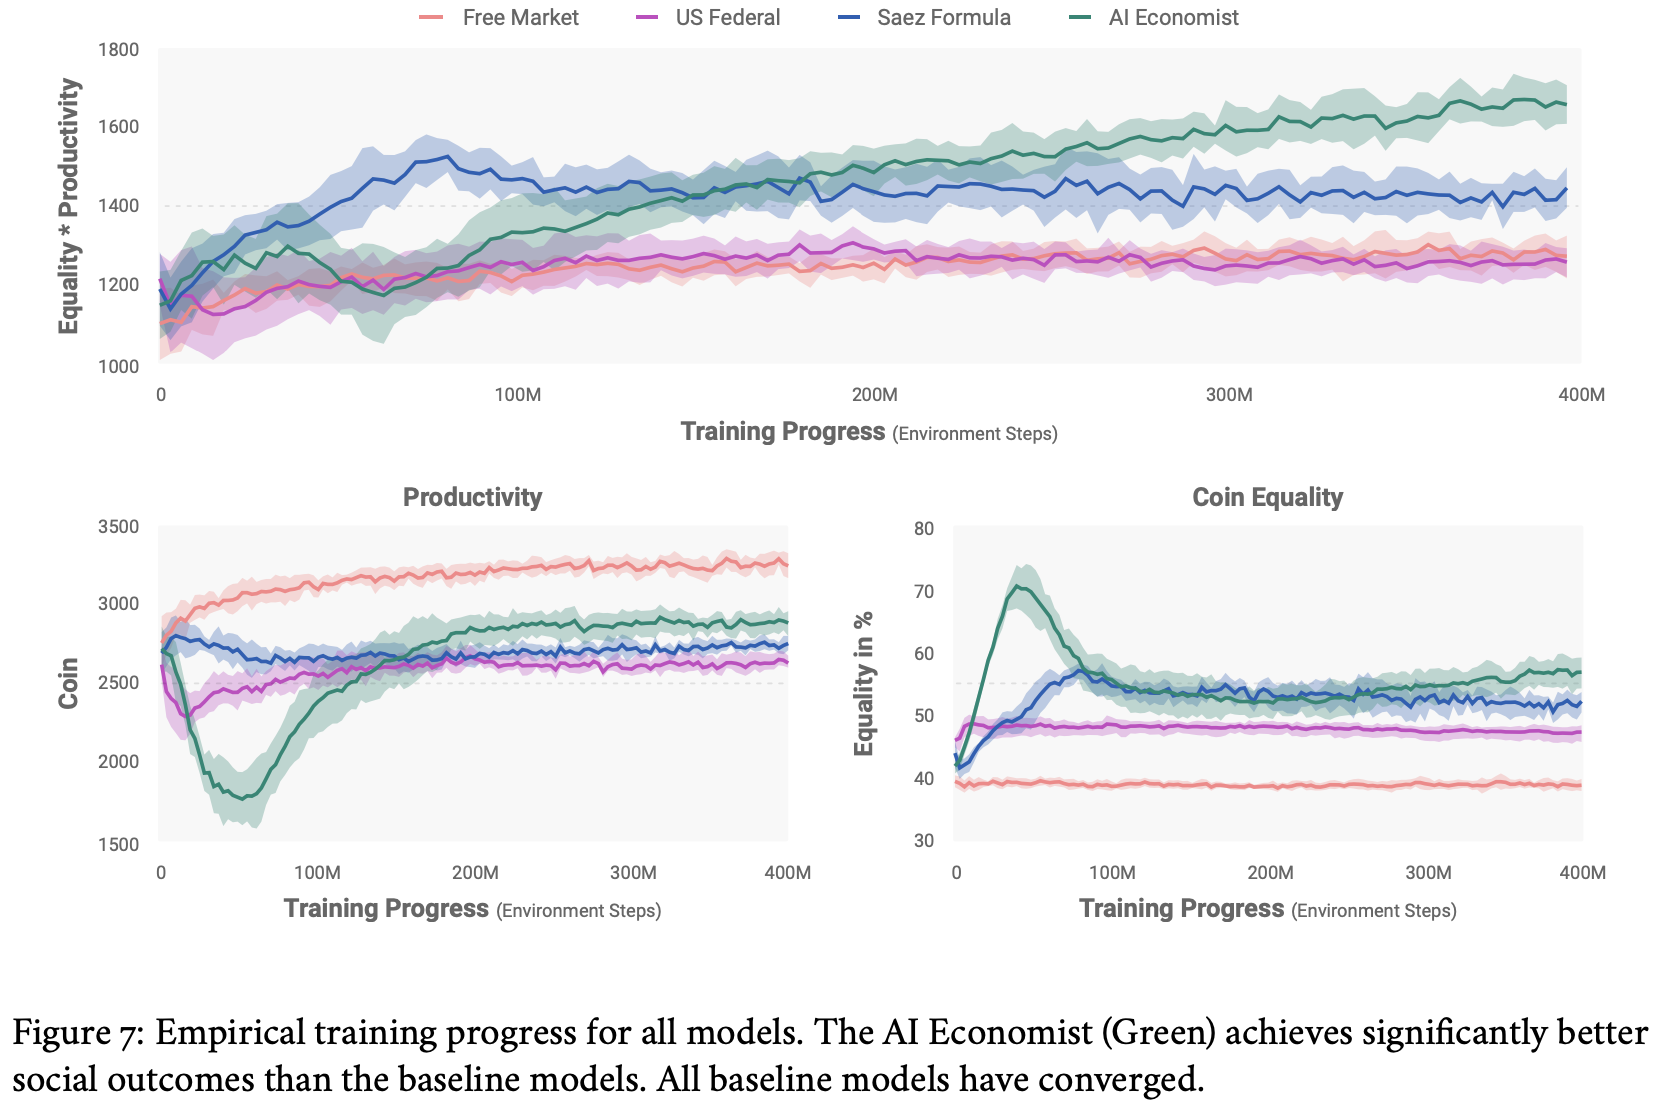
\includegraphics[width=12cm]{figure7.png}
    \end{center}
\end{frame}

\subsection{4.4 Tax Schedules and Wealth Redistribution after Taxes and Subsidies}
\begin{frame}{4.4 Tax Schedules and Wealth Redistribution after Taxes and Subsidies}{}
    {\bf Comparing Tax Schedule}
    \begin{columns}
        \begin{column}{0.5\textwidth}
            \begin{center}
                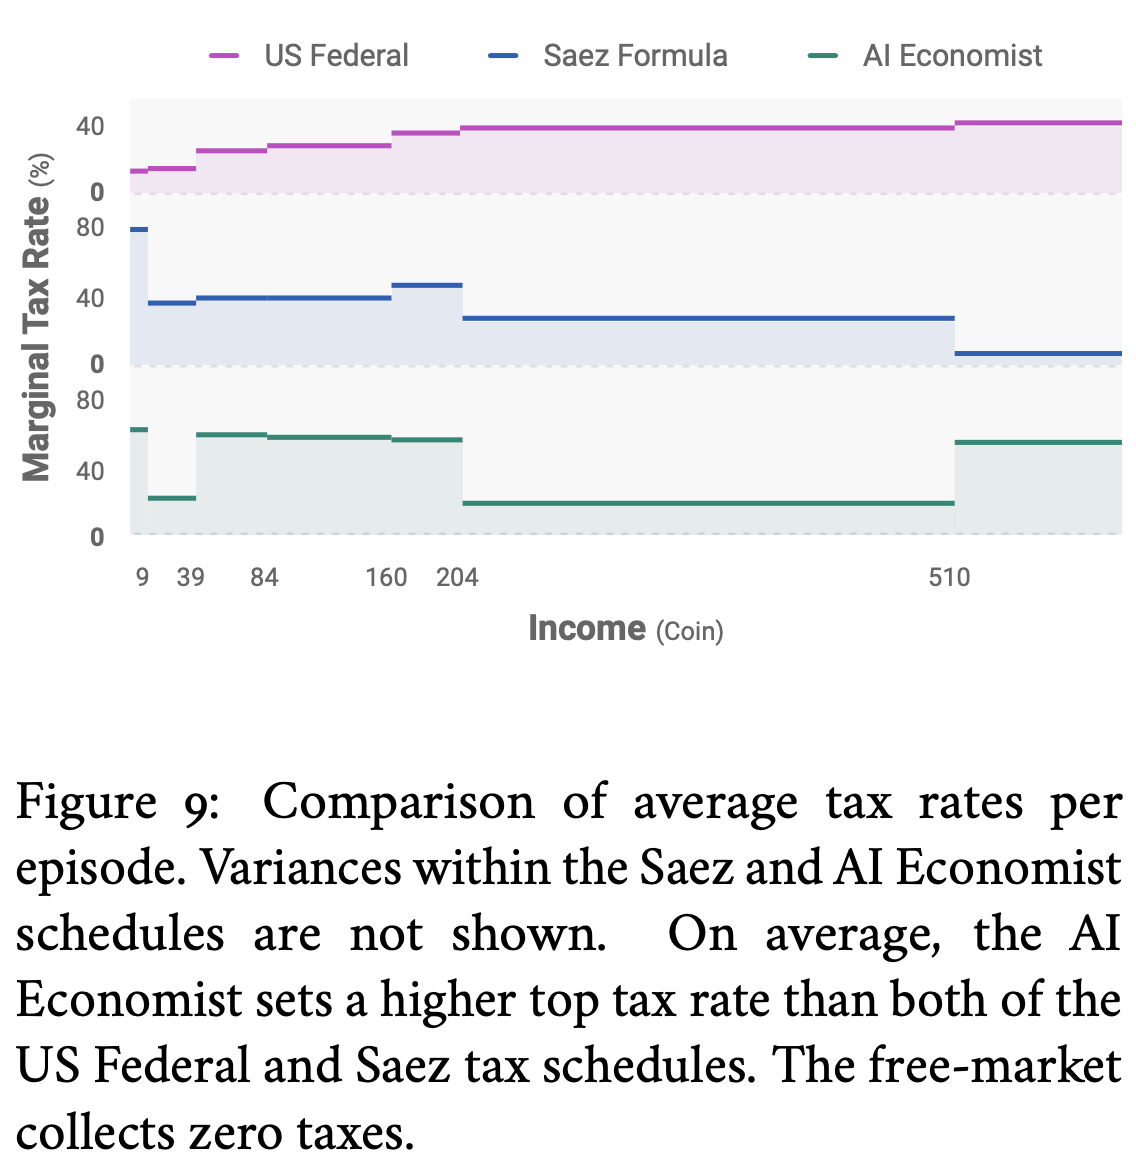
\includegraphics[width=6cm]{figure9.png}
            \end{center}
        \end{column}
        \begin{column}{0.5\textwidth}
            \begin{itemize}
                \item Figure 9は, 各tax modelでのmarginal tax rateの比較.
                \item US federalは, higher incomeに対してmarginal tax rateは上がっていく.
                \item Saez formulaでは概ね逆.
                \item AI Economistはそのblendになってる.
            \end{itemize}
        \end{column}
    \end{columns}
\end{frame}

\begin{frame}{}{}
    {\bf Effective Tax After Redistribution.}
    \begin{center}
        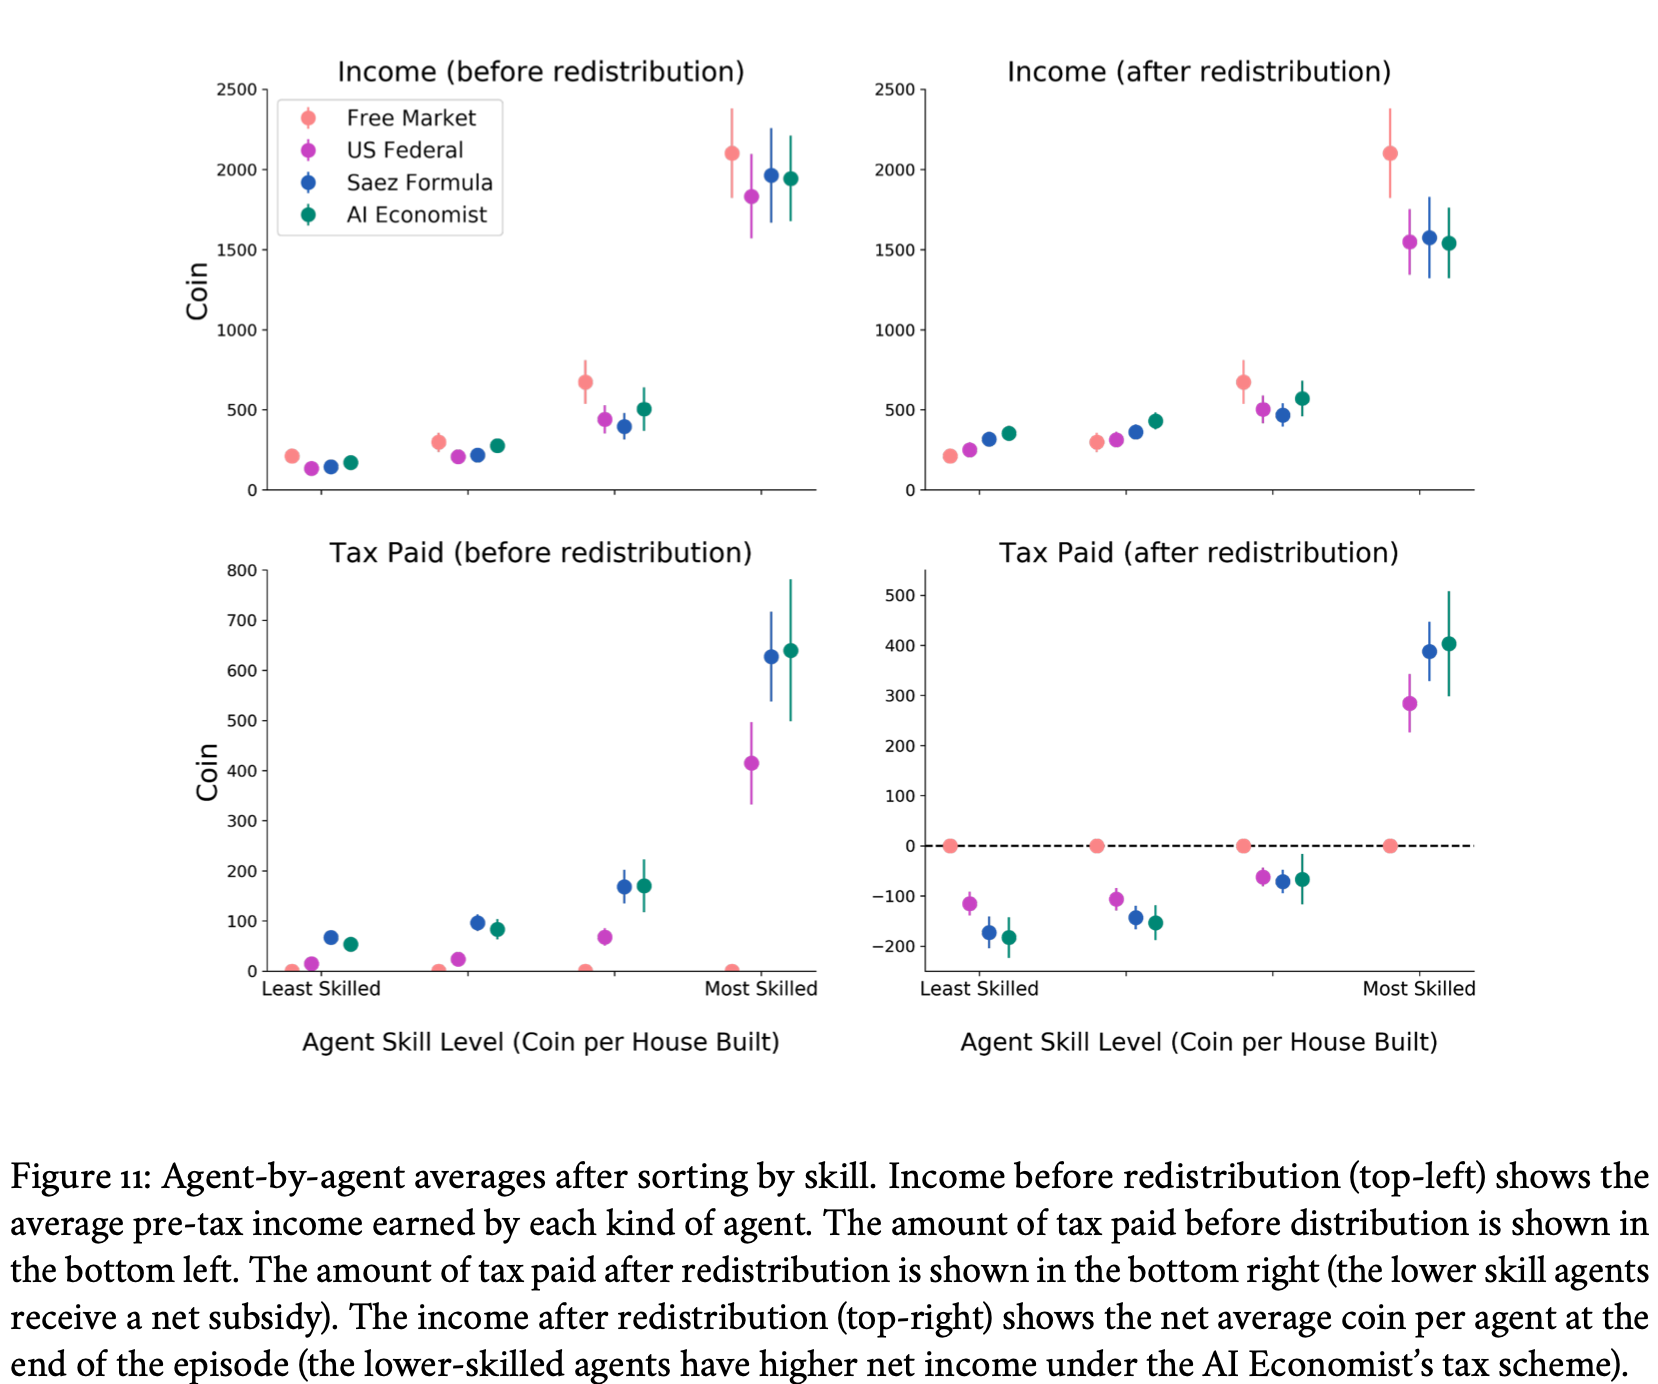
\includegraphics[width=10cm]{figure11.png}
    \end{center}
\end{frame}

\begin{frame}{}{}
{\bf The Impact of Tax on Economic Activity}
\begin{center}
    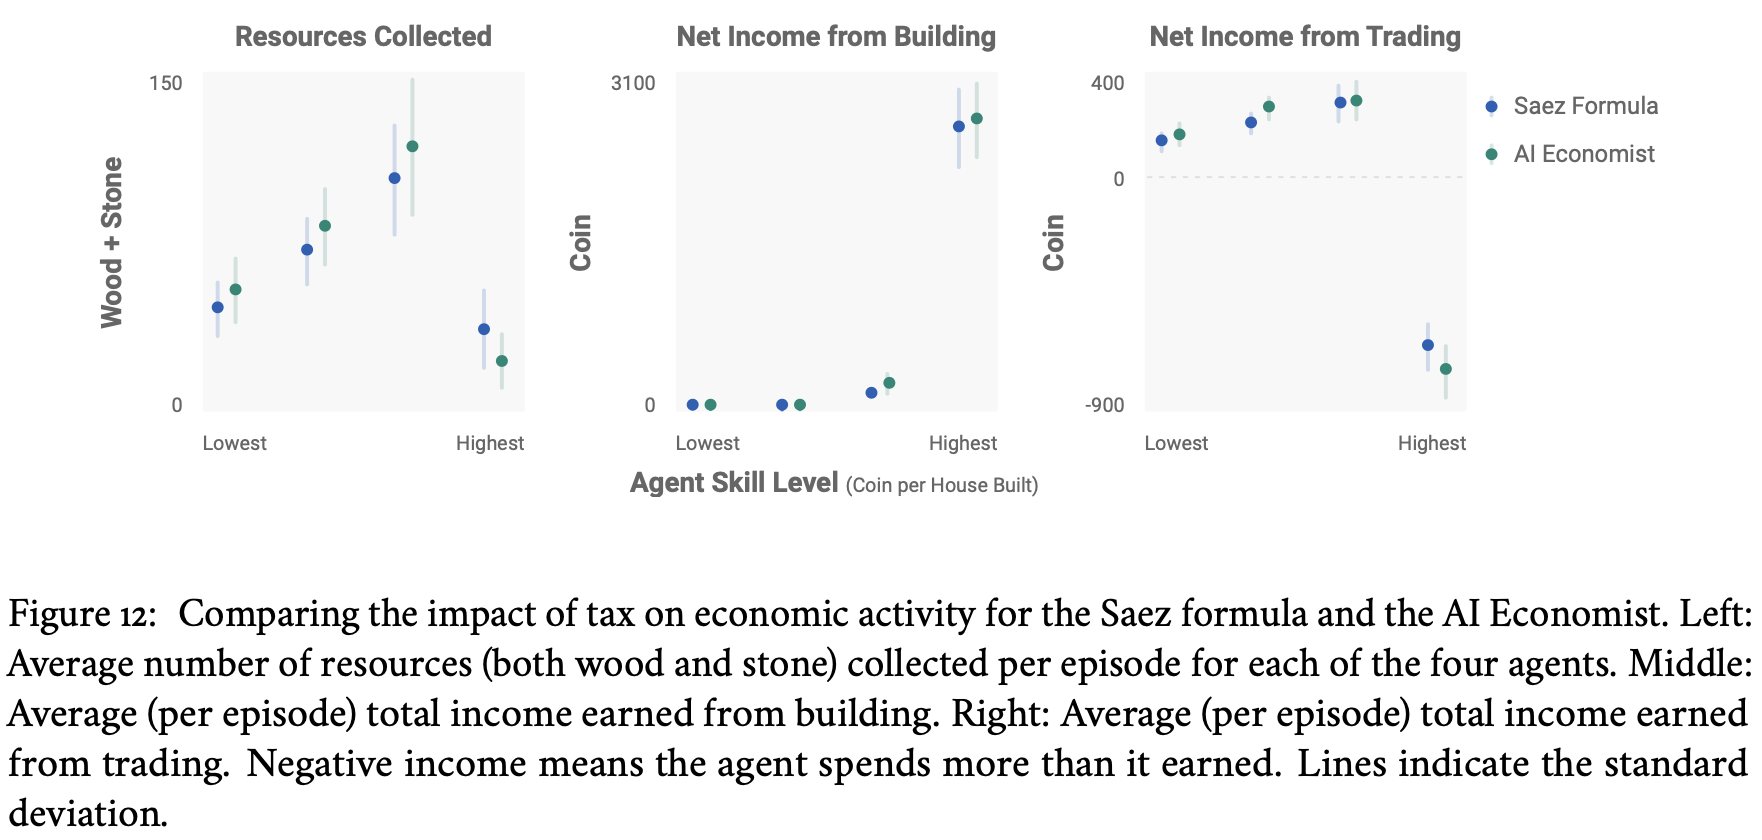
\includegraphics[width=10cm]{figure12.png}
\end{center}
\begin{itemize}
    \item Figure 12は, Saez frameworkとAI economistでのagentの行動の比較.
    \item AI economistでは, high-skill workerはより資源を集めることより買ってbuildingすることに特化し, low-skill workersはより資源を集めるようになっている.
\end{itemize}
\end{frame}

\begin{frame}{4.5 Tax-Gaming Strategies}{}
    \begin{center}
        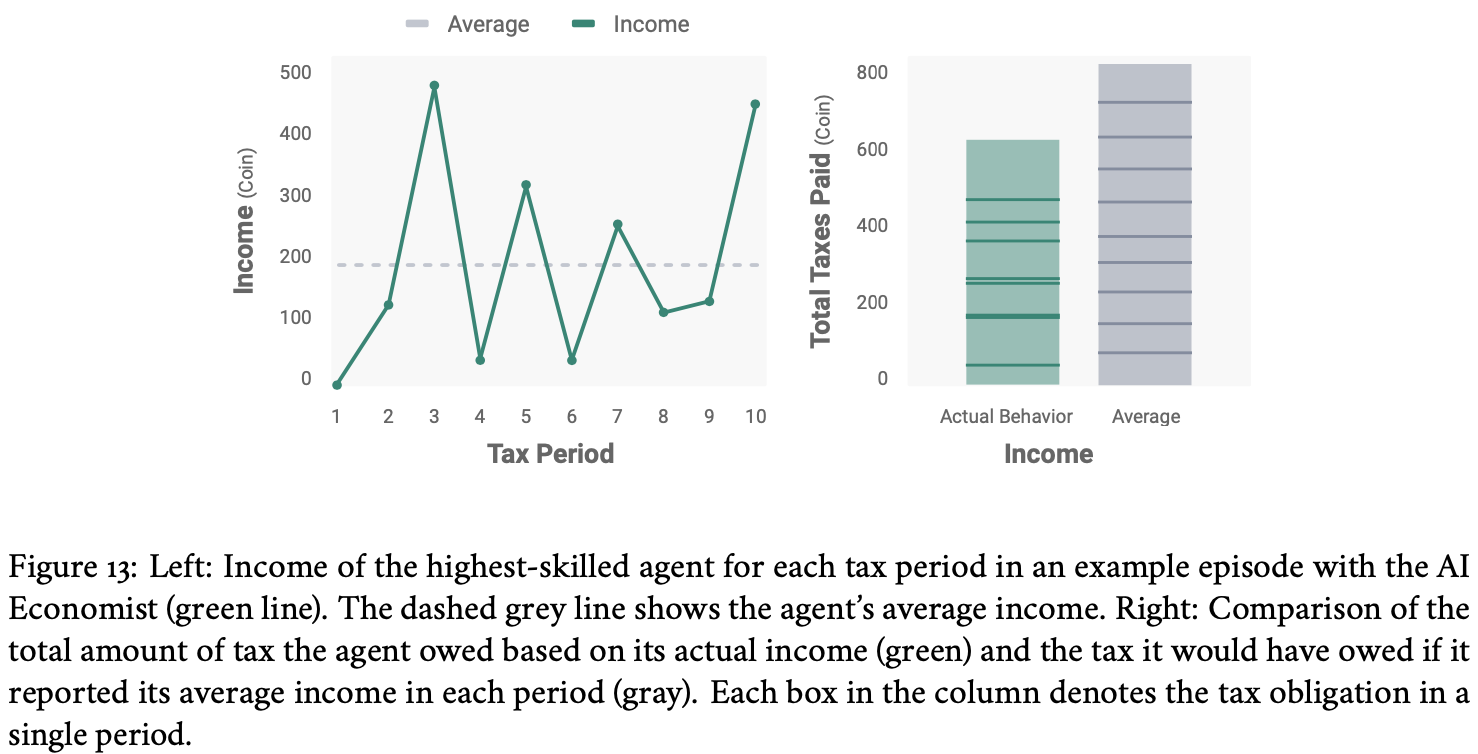
\includegraphics[width=11cm]{figure13.png}
    \end{center}
    {\footnotesize\begin{itemize}
        \item Figure 13はAI economistでのhigh-skilled workerの1 episodeのincomeの推移.
        \item 高収入のtax periodと低収入のtax periodが交互に起きている.
        \item Agentは収入をばらつかせることで課税額を抑えるように行動している(Saezでも)
    \end{itemize}}
\end{frame}
\end{document}